\chapter{Related Work and Background} % Main chapter title

\label{chapter:relatework} 

In this chapter, we first introduce several game genres that we will constantly refer to in the rest of this dissertation, then we review theories studying player engagement and the relationship between player engagement and competence. Next, we review existing endeavors in adaptive techniques which are potential of improving player engagement in video games, and in particular, recommendation systems. Finally, we review churn prediction models which quantify and predict player engagement and will be critical components in our proposed opponent recommendation system.

\section{Game Background}

\subsection{Collectible Card Games (CCGs)}\label{sec:background_ccg}
 We introduce the background for \textit{Collectible Card Games} (CCGs), the testbed for studying starting item recommendation in one-vs-one settings in Chapter~\ref{chapter:qdeckrec}.
 
CCGs have been popular since the 90s, evidenced by the large player base of these kinds of games. For instance, \textit{Magic: the Gathering} has more than 20 million players globally~\cite{guinnessmagic}, while an online free-to-play CCG \textit{Hearthstone} (Blizzard Inc.) reached a record of 40 million registered accounts in 2016~\cite{hearthstonepopular}.  

A CCG typically has hundreds to thousands of different cards, each of which supports specific in-game rules and effects. When playing CCGs, before each match, every player is asked to build a \textit{deck} comprising of a subset of all available cards. While in game, each player takes turns to draw cards from their respective deck and place them on the game board to fare (e.g., attack, counter-attack, cast spell, etc.) against their opponent cards. Cards can be mainly categorized as \textit{spells} and \textit{minions}. Spells are played, creating an effect on the battlefield, and then are discarded. Minions, on the other hand, stay in play, and can be used to attack the opponent or other minions. 

In a match, each player is initialized with certain health points. A match terminates by certain criteria, for example, whenever a player's health is destroyed. Each player is also associated with a certain amount of resource in each turn. A card is only allowed to be played according to its associated rules, e.g., a card can be played when another card is present in hands and the player has resource sufficient over a threshold. A player's turn ends when he or she has no available cards to exert or voluntarily relinquishes the turn. A typical game flow of one-vs-one CCGs is shown in Algorithm~\ref{alg:ccg_1on1}. CCGs are match-based games because any actions in previous matches do not affect upcoming matches: in every new match both players' status get refreshed, such as health, resources, and their decks.


%Algorithm~1 shows the typical game flow of the CCG. 
\begin{algorithm}
    \SetKwInOut{Input}{Input}
    \SetKwInOut{Output}{Output}
    \Input{$Player 1$, $Player 2$ with their customized decks}
    \BlankLine
    
    \While{game not end} {
    \BlankLine
	$curPlayer \leftarrow \text{alternate between } Player1 \text{ and } Player 2$ 
    
    \BlankLine
	$curPlayer$ draws cards from his or her own deck  
 
  	\BlankLine
    $curPlayer$ uses the cards in hands and in play to interact with the game
   		
  	\BlankLine 	
    }
    \caption{Game flow of one-vs-one CCGs}
    \label{alg:ccg_1on1}
\end{algorithm}


In general, there is no single deck which can universally win against all other decks because CCGs often design cards with sophisticated synergistic and oppositional relationships. For example, in Hearthstone, there are two distinguished types of decks that counter each other in different phases of a match. An \textit{Aggro} deck is considered as an aggressive archetype built with cards capable of dealing damage to the opponents as quickly as possible. In contrast, a \textit{control} deck is the opposite archetype with cards which can survive long enough to triumph in the late game through powerful but expensive cards or complex combos.

The goal of deck building (or deck recommendation) is to identify a winning-effective set of cards which suits the player's own play style and effectively counters a target opponent. As deck building is regarded as a crucial part of game play, there exist many online forums and websites for players to discuss, analyze and test deck building strategies (e.g.,~\cite{hearthpwn,icyveins}). However, deck building has a large and complex solution space and thus poses great challenges to players. For example, the number of all possible decks in our experiment setting (Section~\ref{sec:qdeckrec_exp}), which selects 15 out of 312 cards, is $1.4 \times 10^{25}$. 


Although the opponent's deck is invisible to the player during matches, we assume a deck recommendation system can access to any player's deck. This assumption will be used in Chapter~\ref{chapter:qdeckrec}, where our proposed deck recommendation system will search for winning-effective decks against specific opponent stereotypes. 


\subsection{Multiplayer Oline Battle Arena (MOBA)}
Next, we introduce Multiplayer Online Battle Arena (MOBA) games since in Chapter~\ref{chapter:draftart} we will use MOBA games as the testbed for studying winning-effective hero recommendation in a team-vs-team setting.

MOBA is one of the most popular contemporary e-sports. Games such as \textit{League of Legends} (Riot Games) and \textit{DOTA 2} (Valve Corporation) have attracted millions of players to play and watch~\cite{lol_fanbase,lol_27million}. MOBA games have also attracted a variety of research thanks to their complexity and design richness. Some research problems of interest include team formation analysis~\cite{pobie1,pobie2,neidhardt2015team,kim2016proficiency}, skill analysis~\cite{zhengxing2016player,Drachen:skill}, and hero pick recommendation systems~\cite{summerville2017reco,hanke2017reco}. A recent trend also attempts to build AI bots that can play at professional human level~\cite{openaidota}. 

In a classic match of such games, two teams, each composed of five players, combat in a virtual game map (Figure~\ref{fig:moba_map}), the goal of which is to beat the opposite team by destroying their base. Each player controls an in-game character, known as \textit{heroes}~\footnote{We follow the terminology of DOTA 2.}, to co-operate with other teammates in attacking opponents' heroes, armies, defensive structures, and ultimately base, while defending their own in-game properties. We will keep referencing in-game characters as heroes in MOBA games going forwards, as this term is widely accepted by the player community. MOBA games are match-based games~\cite{guo2012analysis} as our definition in Section~\ref{chap1:motiv}, because they are played match by match: a new match starts with random 10 online players and ends whenever a team destroys the other's base, and in-match records from previous matches do not affect a new match, e.g., every player in the new match starts with level one of his or her character, the same amount of golds, and an empty item inventory.


\begin{figure}
\centering
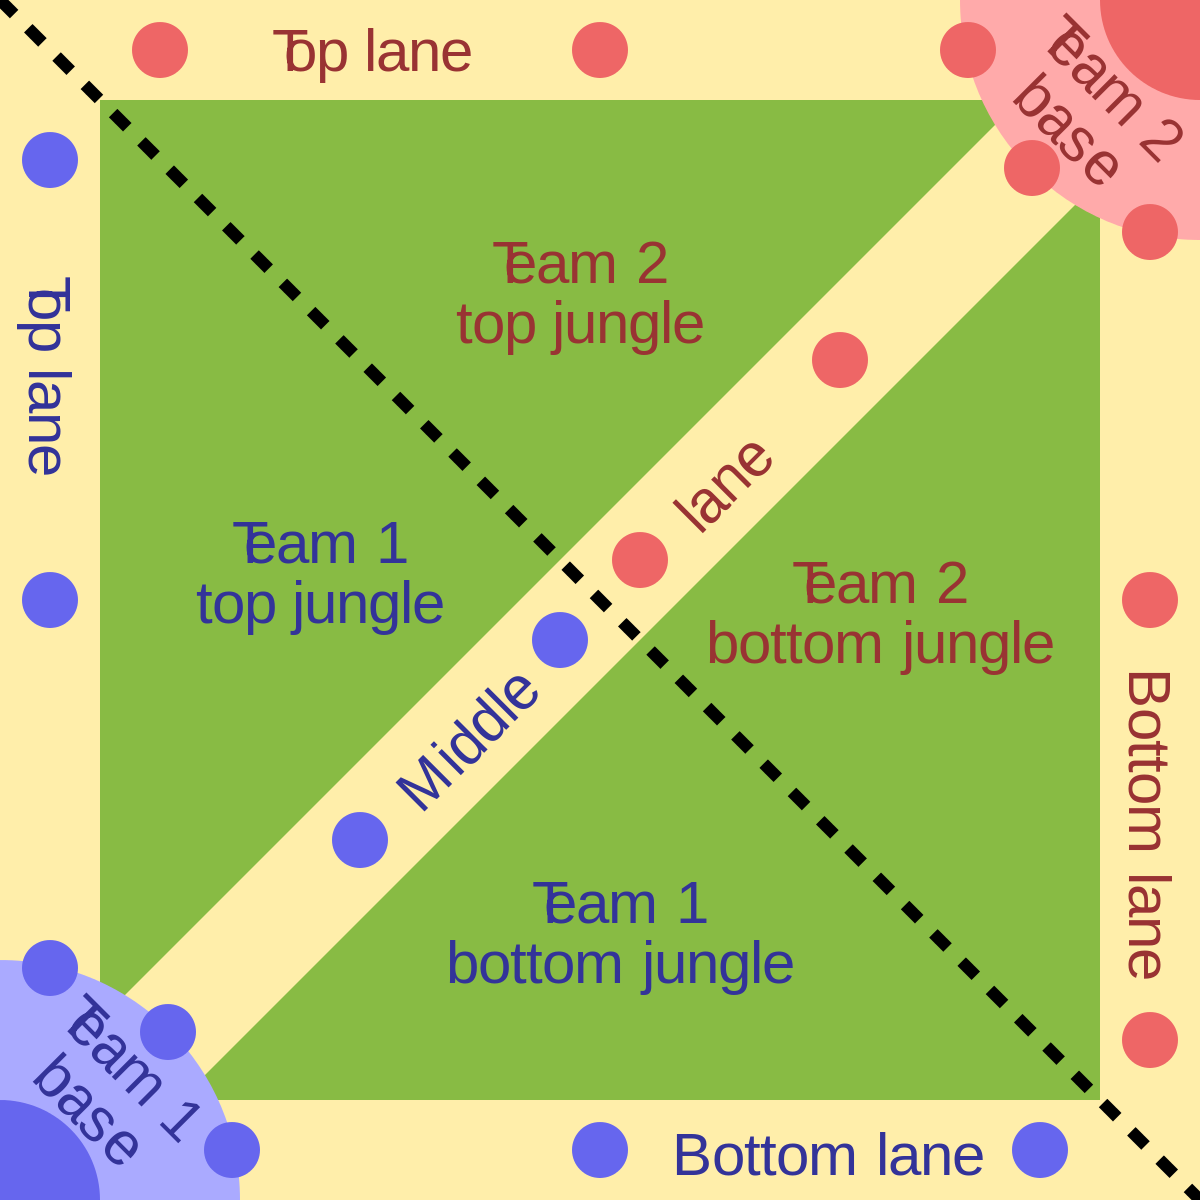
\includegraphics[width=0.6\textwidth]{Figures/map_of_dota.png}
\caption{The game map of DOTA 2. The bases of the two teams are on the ends of the diagonal. Player-controlled characters can move through lanes (Top, Bottom, and Middle) as well as partial areas of jungles. Most MOBA games have similar game maps like this one. Figure downloaded from the Internet: \url{https://bit.ly/2LbD3dv}}
\label{fig:moba_map}
\end{figure}

\begin{figure}
\centering
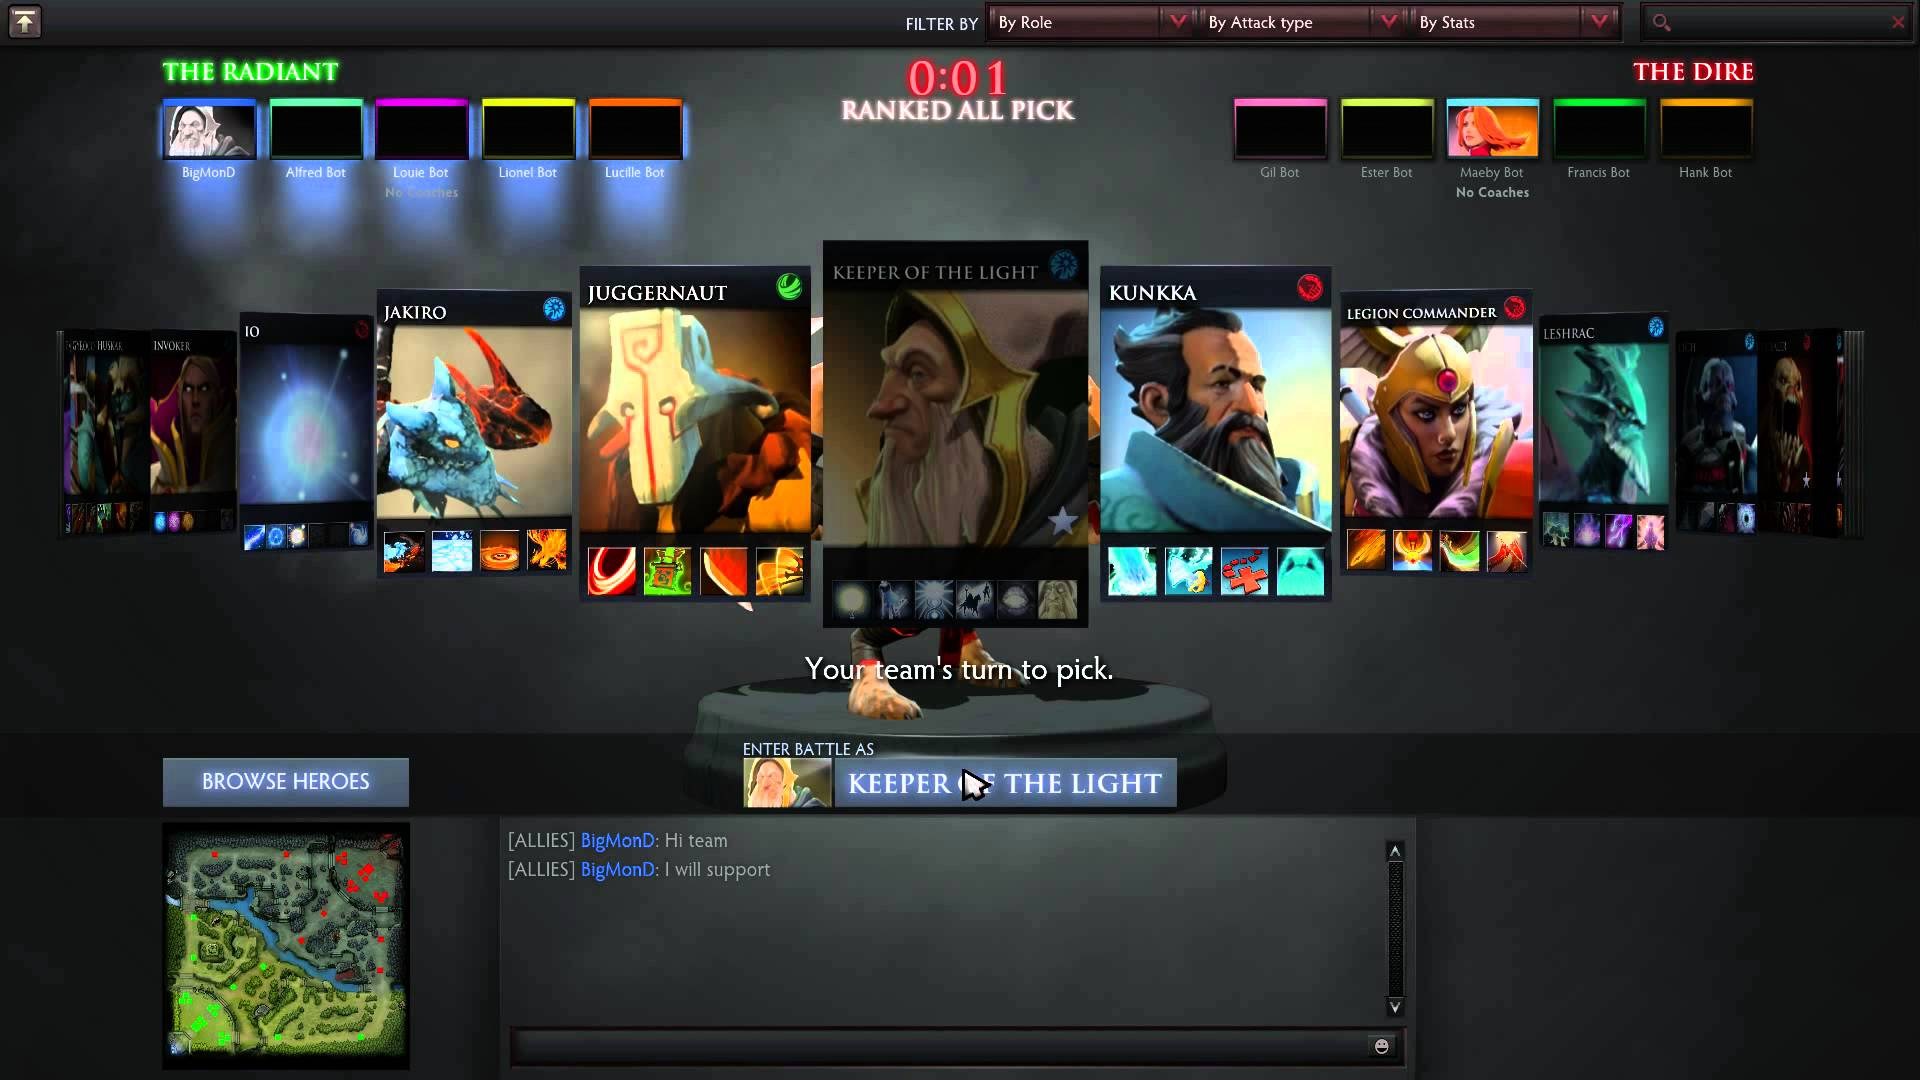
\includegraphics[width=1\textwidth]{Figures/ranked_all_pick.jpg}
\caption{Drafting interface in DOTA 2. Figure downloaded from the Internet: \url{https://bit.ly/2uBY8ni}}
\label{fig:ranked_all_pick_interface}
\end{figure}

Heroes are often designed with a variety of physical attributes and skills, e.g. dealing long-distance damage, healing teammates, or spearheading with strong shields, which together add to a team's overall power. Moreover, there exist sophisticated synergistic and oppositional relationships between heroes. For example, in DOTA 2, hero \textit{Clockwerk} has high synergy with \textit{Naix} because \textit{Clockwerk} can transport \textit{Naix} to target enemies directly, making up for \textit{Naix}'s limited mobility in fighting. In another example, hero \textit{Anti-Mage}'s mana burn skill reduces an opponent's mana resource, making him a natural opposition to \textit{Medusa}, the durability of whom is completely reliant on how much mana she has. Previous research has also highlighted that interactions between heroes greatly influence match outcomes~\cite{pobie1,Semenov2016,kim2016proficiency}, as well as many online discussions about hero pick strategies \footnote{\url{http://www.weskimo.com/a-guide-to-drafting.html}}\textsuperscript{,}\footnote{\url{https://www.reddit.com/r/learndota2/comments/3f9szo/how_to_counter_pick_heroes/}}. 
 
 
The selection of heroes, also known as \textit{pick} or \textit{draft}, takes place before each match starts and alternates between two teams until each player has selected one hero. We refer to the 10 heroes in a completed draft as a \textit{hero line-up}. In a popular match mode named \textit{Ranked All Pick}, the alternating order of drafting is ``1-2-2-2-2-1'', meaning that the first team picks one hero, followed by the second team picking two heroes, then the first team picking two heroes, and so on. The process ends with the second team picking their last hero. During a draft, heroes already selected are visible to both teams. Heroes can only be selected from a fixed pool and no duplication is allowed in the same match. Moreover, a time limit (usually a few dozens of seconds) is imposed for each hero pick. Figure~\ref{fig:ranked_all_pick_interface} shows the interface for drafting in DOTA 2, where in the central area a gallery of available heroes is presented for selection. In games like DOTA 2, there are possibly more than 100 heroes that can be picked by a player at the time of drafting. As estimated by~\cite{hanke2017reco}, the number of possible hero line-ups in DOTA 2 is approximately $1.56 \times 10^{16}$. There are more sophisticated drafting mechanics and rules deployed and interleaved with hero picks in other match modes, such as \textit{banning} (i.e., certain heroes can be prohibited from selection by either team). To make illustration easier and simpler, we will assume we study under Ranked All Pick mode unless otherwise mentioned in Section~\ref{sec:draftart_extension}.

Due to the complex synergistic and oppositional relationships among heroes and large numbers of follow-up pick possibilities by other players, as we described above, the hero drafting phase becomes a critical component contributing to match outcomes even though it happens before the real match starts, and selecting a winning-effective hero is a challenging task to human players especially those inexperienced~\cite{johnson2015all}. 




\section{Theories of Player Engagement and Competence}

The primary motivation of this dissertation is to improve player engagement. A straightforward way to define player engagement is the "continued desire" to play the game repeatedly during play or over a longer period of time~\cite{schoenau2011player}. Player engagement as a complex construct has been extensively studied in many theoretical frameworks and linked to numerous aspects, such as happiness~\cite{sweetser2005gameflow,flow1990psychology,chen2007flow}, motivations~\cite{przybylski2010motivational,ryan2006motivational,yee2006demographics,yee2006motivations,sherry2006video}, presence~\cite{lombard1997heart,tamborini2006role}, immersion~\cite{mcmahan2003immersion,brown2004grounded,jennett2008measuring,ermi2005fundamental}, pleasure~\cite{costello2009tool}, enjoyment~\cite{ravaja2007fun,klimmt2003dimensions,mekler2014systematic}, fun~\cite{koster2013theory} and playability~\cite{federoff2003improving,federoff2002heuristics,desurvire2004using,nacke2009playability}.

One trigger for player engagement which has been extensively studied is in-game challenge and competence, which means player enjoy the experience of victory, accomplishment or dominance over other players while being appropriately challenged~\cite{ryan2006motivational,przybylski2010motivational,yee2006motivations,wu2010falling,sherry2006video,lazzaro2004we,schoenau2011player}. One foundation to study player competence and engagement is theory of motivation. Within this body of work, Self-Determination Theory (SDT)~\cite{ryan2000self}, a widely researched framework for the study of human motivation, has provided support for the importance of competence to drive player engagement. In more details, SDT proposes that the nutriments for healthy development and functioning are three basic psychological needs for \textit{autonomy} (the sense of volition or willingness when doing a task)~\cite{deci2000and,deci1964empirical}, \textit{competence} (the need for challenge and the feeling of being capable and effective)~\cite{white1959motivation,deci1985intrinsic}, and \textit{relatedness} (the feel of being connected with others)~\cite{ryan2001happiness,la2000within}. When the psychological needs are satisfied, people will develop positive altitude and act effectively and hence experience well-being; however if they are thwarted, people will more likely conduct negative behavior, such as prejudice and aggression. ~\cite{ryan2006motivational,przybylski2010motivational} later extend SDT to the activity of playing video games and verify that the three pillars of intrinsic needs (autonomy, competence, and relatedness) also hold for motivating people engaged in playing games. 

Other theoretical works examining motivations underlying video game playing also discover similar needs for competition and challenge. The principle component analysis by~\cite{yee2006motivations} reveals three overarching motivation components (Achievement, Social, and Immersion); competition referring to the desire to challenge and compete with others is nested under the Achievement component. \cite{wu2010falling} verify Yee's three motivation components in the perspective of Uses and Gratification (U\&G) theory~\cite{palmgreen1985uses}, which posits that users actively seek out specific media that gratifies their specific needs. \cite{wu2010falling} find that players' continuation motivation is significantly impacted by the perception of gratification (i.e., Achievement, Social, and Immersion). Also dwelt in the U\&G theory, \cite{sherry2006video} identify 6 different gratifications of video game use, including challenge and competition along with social interaction, diversion, fantasy, and arousal. \cite{lazzaro2004we} proposed four keys to release player emotions during play: Hard Fun, Easy Fun, Altered States, and the People Factor; Hard Fun refers to game challenges which frequently elicit emotions and experiences such as frustration and Fiero. \cite{schoenau2011player} explains player engagement as a process whereby players could feel positive affect through accomplishment (achievement, progression, and completion) and in turn be motivated to continue playing.  

Furthermore, players do not simply look for in-game challenge and competence, but those commensurate with player skills, as indicated by the Flow theory~\cite{flow1990psychology}. The Flow theory has been studied by its author for long since mid-1970s in an attempt to discover major components for universally explaining why people immerse in their tasks despite of different occupations; Flow refers to the optimal mental state of engagement when people get fully immersed, concentrated, and enjoyed in their activities and lose track of time~\cite{flow1990psychology}. \cite{sweetser2005gameflow,chen2007flow} adapt the Flow theory to video games and identify that that there should be an optimal match between the skills a player possesses and the challenges presented by the game in order to achieve optimal engagement. 

The theories introduced above provide substantial support that providing proper competence to players will lead to better player engagement, which constitute the hypothetical foundation for our works to recommend winning-effective in-game elements as we assume that those players being incapable of selecting winning-effective in-game elements could regain competence if adopting our recommendations. 


\section{Techniques towards Improving Player Engagement}

Here we introduce three kinds of techniques related to our dissertation: Dynamic Difficulty Adjustment (DDA)~\cite{hunicke2005case}, Procedural Content Generation (PCG)~\cite{yannakakis2011experience,togelius2011search} and Recommendation System~\cite{medler2011using}. 

% Inspired by the theoretical works on player competence and  engagement introduced above, two forms of techniques have been mainly used, based on our literature review, for manipulating player competence: dynamic difficulty adjustment (DDA) and recommendation systems.

DDA manipulates game difficulty adaptively via various techniques~\cite{hunicke2005case}, with the goal to keep players' perceived competence stay in the optimal zone of flow~\cite{flow1990psychology,sweetser2005gameflow,chen2007flow}. Procedural Content Generation (PCG) techniques~\cite{yannakakis2011experience,togelius2011search} refers to automatically (or algorithmically) generate adaptive in-game content. Recommendation systems are used as information filtering tools to dedicatedly present specific in-game elements from a pool of candidates~\cite{medler2011using}; however, different than PCG, candidates of in-game elements are assumed to have been generated already by the game.

DDA is related to our dissertation because recommendations of winning-effective in-game elements, which we study in \hyperref[rq1]{\textbf{R.Q.~1}}, may also cause the difficulty and player competence change if players adopt the recommendations. Therefore, in our opinion, techniques we will investigate to answer \hyperref[rq1]{\textbf{R.Q.~1}} are also within the radar of DDA. PCG is related to our dissertation because  recommendation systems and PCG are both valid methodologies to influence player competence and engagement. The difference is that PCG requires the access to directly modify the game content, while recommendation systems do not - recommendation systems access and filter on  \textit{generated} game content. 

While PCG and recommendation systems are named under their methodologies, DDA is named under its goal (i.e., to adjust difficulty). Therefore, DDA actually involve various techniques including PCG and recommendation systems. And PCG and recommendation systems can be used for various goals including DDA. In the following, we introduce each of these techniques.






\subsection{Dynamic Difficulty Adjustment}

A straightforward way to manipulate game difficulty is \textit{rubber banding}, which means the difficulty of the game rises or falls if the player plays well or poorly. A famous example is from \textit{Mario Kart} series (Nintendo Co., Ltd), in which players who lag behind are more likely to get power-ups for speeding up and attacking front runners. Rather than having an monotonous approach of difficulty adjustment for all players, some more advanced works leverage player modeling~\cite{yannakakis2013player} as a powerful tool to identify more granular players' preferences and deliver more personalized difficulty adaptation~\cite{missura2009player,togelius2006making,yannakakis2005player,zook2012temporal}. Another notable kind of advanced models is to formulate difficulty adjustment in a more rigorous probabilistic framework: \cite{missura2011predicting} formulate adjusting difficulty as an online learning problem~\cite{auer1995gambling} in which the difficulty ranking of finite game difficulty settings is estimated through a trial-and-error fashion with the goal to choose the ``just right'' difficulty setting as often as possible. 

The ways to deliver difficulty adjustment can be as simple as tuning pre-defined parameters which govern environmental changes (e.g.,~\cite{hunicke2005case,baldwin2014effect}), or can be as sophisticated as AI-controlled agents that could adapt to players' gameplay (e.g., the work of~\cite{demediuk2017monte} based on Monte Carlo Tree Search~\cite{browne2012survey}, a series work of Andrade and his colleagues~\cite{andrade2006dynamic,andrade2005challenge,andrade2005extending} based on Reinforcement Learning~\cite{sutton1998reinforcement}, and~\cite{spronck2004difficulty}'s work based on behavioral scripts). 

Several works have conducted experiments and shown that player engagement-related metrics indeed improve due to implemented DDA. In the work by~\cite{hunicke2005case}, the author adjusts supply and demand in a game and finds that expert players report slightly elevated levels of enjoyment while novice players do not. In the work by~\cite{van2009incongruity}, players report to have decreased pleasure and increased frustration when playing harder games compared to balanced games. ~\cite{xue2017dynamic} deploy a difficulty adjustment system to a commercial matching-three game (a game like \textit{Candy Crush}), discovering that difficulty adjustment could bring as much as $7 \sim 9 \%$ improvement in total numbers of rounds played and duration of gameplay. \cite{sarkar2017engagement} find that presenting to players 
tasks in skill-based difficulty ordering led to significantly more attempted and completed levels than random ordering in a crowdsourcing science game. 

\subsection{Procedural Content Generation}

Procedural Content Generation (PCG) is the algorithmic generation of game content with limited or indirect user input~\cite{yannakakis2011experience,togelius2011search}. The goal of applying PCG is not only to eliminate the burden from developers to manually create in-game content, but also adapt game content to satisfy players' dynamic needs. \cite{togelius2011search} provides a comprehensive taxonomy on different types of PCG algorithms, such as online-vs-offline (whether game content is generated during the run time or developement time of the game), random-seeds-vs-parameter-vectors (generation up to a single seed or a series of specifications), etc.

PCG has been used both for adjusting difficulty and player engagement, depending on what the underlying evaluation method is for evaluating generated content. An example of applying PCG for difficulty adjustment is an early work from ~\cite{jennings2010polymorph}, in which levels of a platform game are automatically generated  segment by segment - next segment is generated with the difficulty level appropriate for how the player performs in the current segment, where the mapping from level specifications to difficulty is learned by a machine learning model on real player data. On another platform game, PCG is applied to levels which optimize player engagement, with a player engagement prediction model trained on previous gameplay data used to guide the generation of levels.  

Although PCG and recommendation systems are both valid and potential ways to improve player engagement, we focus on the latter in this dissertation. As we introduce in Chapter~\ref{chapter:intro}, studying PCG would require access to some testbed games for modification of game content, which was not available to me during my research. Therefore, we primarily study recommendation systems which rely on collected data and simulators.

\subsection{Recommendation Systems}
% Rather than directly manipulating in-game elements like DDA, recommendation systems are used as information filtering tools to dedicatedly recommend to players specific in-game elements from a pool of candidates which are assumed to be generated already by the game~\cite{medler2011using}.


Recommendation systems~\cite{isinkaye2015recommendation,bobadilla2013recommender,resnick1997recommender,adomavicius2005toward} have been studied for long in a variety of web applications such as movies~\cite{amatriain2012netflix}, e-commerce~\cite{linden2003amazon} and news~\cite{das2007google}. The video game industry has also used recommendation systems to introduce players games that they are likely to enjoy~\cite{sifa2014archetypal,orland10,skocir2012mars,wu2017recommendation}. These recommendation systems serve as information filtering methods to alleviate information overload faced by users, as users are not able to go through all candidate items usually in a great amount within those web applications. To this end, these traditional recommendation systems predict users' preferences on items accurately such that personalized item recommendations can be given based on the ranking of user preference predictions~\cite{liang2006personalized}. 

Video games as the form of interactive entertainment allow game developers apply recommendation systems not only for recommending next games, but also in-game elements within a game. In this dissertation, we focus on recommendation systems for in-game elements within match-based video games which have distinctive features than traditional recommendation systems introduced in the previous paragraph. First, our goal is centering on predicting in-game elements' influences on winning-effectiveness and engagement, which may be manifested by metrics like winning probabilities, rather than players' preferences on those in-game elements. Second, in-game element recommendations to one player may affect other players' experience. Therefore, in-game element recommendations have to consider other players' information. This is contrastive to traditional recommendation systems where recommended items to one user are relatively independent to other users' experience.

Although recommendation systems have been utilized on a variety of in-game elements for various purposes~\cite{kolen2018horizontal,wu2017recommendation}, those sharing the same scope as this dissertation have only sporadic appearances in literature (i.e., in-game element recommendations in the pre-match stage in match-based games for influencing player competence and engagement). 
Our suspicion for the lack of research in this scope is that accessing to data of large-scale commercial games which have sufficiently sophisticated in-game elements for applying recommendation system techniques is not always easy. The difficulty may drive academic research to focus only on a few publicly accessible datasets or games with a smaller scale of which researchers can have full control. Nevertheless, we survey existing works as follows, with each subsection corresponding to a specific type of in-game element recommendation for answering  \hyperref[rq1]{\textbf{R.Q.~1}} and  \hyperref[rq2]{\textbf{R.Q.~2}}.

% (e.g., starting gifts in Dark Soul and starting weapons in Bloodborne)

\subsubsection{Starting Item Recommendation}\label{sec:rw_startitem}
Starting items are commonly seen elements in a variety of genres of games, such as Action Role-Playing Game (Action-RPG) and Multi-Player Online Arena (MOBA), where starting items aid in-game characters heal, scout, defend, and attack when characters are weak in their initial stages, and Collectible Card Games (CCGs), where starting items refers to a set of cards, called a \textit{deck}, which players need to designate from a pool of candidate cards prior to a match starts and upon which players' in-game abilities and strategies will depend (See CCG background in  Section~\ref{sec:background_ccg}). Some games have incorporated starting item recommendation features; for instance, when making purchases of starting items in League of Legends, players can browse the full list of all items or a short list of recommended items for easier choices~\cite{lol_recomitem}. 

Despite the prevalence of starting items in video games, to our best knowledge, we have only seen little academic research in starting item recommendation. Specifically in the problem of deck recommendation for one-vs-one CCGs, which we will study in Chapter~\ref{chapter:qdeckrec}, we have only seen search-based solutions using either heuristic searches or metaheuristic searches~\cite{birattari2009tuning}. However, neither of the search methods is efficient enough to deploy for large-scale or real-time deck recommendation. 

Heuristic search methods suggest which cards to include in a deck based on domain heuristics such as popularity and in-game resource curve~\cite{frankkarsten,willfancher,stiegler2016hearthstone}. However, they require in-depth human knowledge and lack flexibility to adapt to different play styles and opponents. Metaheuristic searches rely on high-level, problem-independent, approximate search strategies for tackling optimization problems~\cite{birattari2009tuning}. Researchers have used one type of metaheuristic search called \textit{Genetic Algorithm} (GA)~\cite{holland1992adaptation} to evolve decks towards higher winning-effectiveness through repeated modifications and selections~\cite{garcia2016evolutionary,bjorke2017deckbuilding}. In GA~\cite{holland1992adaptation}, candidate solutions (called \textit{individuals}) evolve towards better feasible solutions iteratively with \textit{mutation} and \textit{crossover} operators. In each generation, the \textit{fitness value} of every candidate solution is evaluated. The fitness value is usually the value of the objective function in the optimization problem being solved; in the works of ~\cite{garcia2016evolutionary,bjorke2017deckbuilding}, the fitness value is the average win rate of a candidate deck against a group of opponent decks while AI bots are used as a proxy for human play. The more fit candidate solutions are stochastically selected and modified to form a new generation. Although not requiring human knowledge to guide searches, metaheuristic search algorithms require a large computational cost for simulation-based evaluation on intermediate solutions, which renders them unsuitable for large-scale or real-time usage. In Section~\ref{sec:qdeckrec_existmethodanaly}, we will analyze in details how inefficiency of existing approaches arises. 

\subsubsection{Character Recommendation}\label{sec:rw_character}
The rich design of characters and recent worldwide popularity of MOBA games have allowed them become the primary testbed for character recommendation research. Classic MOBA games like League of Legends and DOTA 2 are usually played 5-vs-5; there are possibly more than 100 characters that can be picked by a player in the pre-match stage. Moreover, as per rules of certain match modes players are supposed to select characters in sequence; players need to consider synergistic and oppositional relationships among champions because a winning-effective character should not only fit to selected characters so far but also projected characters selections by the rest of players. 

To recommend winning-effective characters in the character selection phase, \cite{hanke2017reco} proposed to mine association rules~\cite{agrawal1994fast} from historical character selection data and use them as the heuristic to recommend heroes. Here, association rules are character subsets that appear frequently together either in the winning team or in opposite teams. Any character contained in the discovered association rules together with characters picked already is suggested to be a good candidate to pick next. However, this method does not consider which characters \textit{will} be picked  by other players in the rest of the drafting process, hence this is essentially a myopic, greedy-based approach.

% Previous works on hero pick recommendation can be categorized into two main approaches, based on (1) historical selection frequency, and (2) previous win rate.

Researchers have also proposed to recommend characters based on player selection tendency. \cite{summerville2017reco} models character recommendation as a sequence prediction problem. They train a sequence prediction model for predicting next character which is most likely to be selected next based on historical character selection sequences. However, the predicted character is ``what is
likely to be picked, not what is necessarily best''~\cite{summerville2017reco}. Therefore, character recommendation based on such a method may not be winning-optimal for team victory.

Although there are other works predicting match outcomes~\cite{Yang:identifying,Semenov2016,makarov2017predicting} and analyzing in-game traces~\cite{cavadenti2016did}, they do not focus on how to utilize these models for character recommendation in the context of sequential character selection.


\subsubsection{Matchmaking (Opponent Recommendation)}

% My\'{s}lak and Deja 
% Delalleau et al. 

In practice, the concept of opponent recommendation is often implemented as matchmaking services which connect players to form matches. As such, players themselves become the subjects of recommendations.

% Jim{\'e}nez-Rodr{\i}guez et al.

A fair amount of matchmaking systems simply assume that skill balanced games are good for engagement \cite{graepel2006ranking,sweetser2005gameflow,flow1990psychology,chen2007flow} and hence resort to skill rating algorithms~\cite{glickman1999parameter,elo1978rating,herbrich:trueskill} to identifying similarly skilled opponents. \cite{myslak2014developing} suggests additional information about player preferences in in-game avatar roles can further improve fairness-based matchmaking systems. A few researchers have explored methods to improve player engagement through matchmaking. \cite{Delalleau2012} proposed to train a neural network based architecture which predicts player enjoyment based on their historical statistics. They measured enjoyment by directly asking players for feedback after each match. However, their enjoyment-based matchmaking has not been verified in real games. Plus, whether players are willing to give feedback about enjoyment and how reliable their feedback would be are questionable. \cite{jimenez2011matchmaking} proposed that matchmaking could be based on preferred roles by players. They argue that a fun match should have players act in  roles with perceivably joyful role distribution. However, it is still a conceptual, heuristic-based method without experiment showing that such matchmaking system indeed improves concrete engagement metrics. To our best knowledge, we have not seen any existing opponent recommendation method that formally treats the opponent recommendation task as an optimization problem to maximize player engagement. 




\section{Prediction Models for Player Engagement and Churn}


Player engagement prediction will serve as an important building component in our proposed opponent recommendation work in Chapter~\ref{chapter:eomm}. Player engagement naturally derives from user engagement prediction, which has been applied within various disciplines for decades, such as telecommunications \cite{ferreira2004data}, online advertisements \cite{yoon2010prediction} and insurance \cite{morik2004analysing}. 

Video games have also sparked a number of studies in player engagement modeling and prediction recently due to increasing collection of player data and adoption of data analysis models. In these studies, player engagement are embodied by many specific metrics, such as purchases in the game~\cite{xie2015predicting,sifa2015predicting}, the number of matches played within a time window~\cite{xue2017dynamic,weber2011modeling}, or churn risk~\cite{hadiji2014predicting,harrison2012players}, defined as the proportion of total players stopping playing the game over a period of time. We note some representative player engagement models. Weber~et~al.\! \cite{weber2011modeling} built a regression model to predict the number of games played. They also used the model to aid game design by identifying the most influential features on player retention. Hadiji~et~al.\! \cite{hadiji2014predicting} established the fundamental in churn prediction in free-to-play (F2P) games by suggesting definitions of various churn behaviors, proposing universal behavioral telemetry, and comparing different machine learning models across five commercial F2P games. Runge~et~al.\! \cite{runge2014churn} not only trained a churn prediction model for a casual social game but also showed how the game can leverage the model to increase the effectiveness of promotions to players. \cite{bertens2017games} propose a scalable algorithm using conditional inference survival ensembles~\cite{hothorn2006unbiased} to predict both the level and accumulated time when a player leaves the game.



% Each CCG has a fundamental set of rules that describes the players' objectives, the categories of cards used in the game, and the basic rules by which the cards interact. The CCG that we will use is 1-vs-1 and turn-based. In a match of the CCG, two players take turn to make movements. Each player is initialized with certain health points. The victory objective is to destroy the opponent's health by playing the cards in possession. Each player is also initialized with certain mana points. Mana points get refresh in each turn and increase as the game proceeds. One card is drawn from the player's \textit{deck} to his hands at the beginning of his each turn. Deck is a collection of cards that the player selects from an available pool of cards before the match starts. After the draw, the player uses the cards he has drawn to his hands to interact with the game in order to gain an advantage over the opponent. Each card is assigned with a fixed mana cost. When a card is played out of his hands, it costs the designated amount of mana from the player. The player's turn ends when he has no available actions to perform or he voluntarily relinquishes his turn. 

% Each card is associated with effects, attributes and rules to play it. There are two types of cards, \textit{Minion} and \textit{Spell}. Minion cards, when cast from the player's hands, stay in the game helping the player attack and defend until the opponent takes actions to eliminate them. Spell cards will adjust the game environment as per their designated effects, for instance, one-time damage to opponent or his minions, or recover health to the player or his own minions, or summon new minions. 

% Deck is the initial equipment in CCGs. Because the size of total available cards (usually hundreds or thousands) is much larger than the size of deck (usually a few dozens), CCG players need to strategically customize their decks to take advantage of favorable card interactions, combinations and statistics. However, some inexperienced players have too limited knowledge to construct a competent deck to win a match. 

% Therefore, players need to draft heroes that can enhance the strengths and compensate for weaknesses of teammates' heroes (i.e., \textit{synergy}), while posing suppressing strengths over those in the opponent team (i.e., \textit{opposition}).

% The pursuit of victory and achievement is a common reason of player engagement~\cite{schoenau2011player,yee2006motivations,sherry2006video,wu2010falling,lazzaro2004we}. Victorious or progressive game outcomes can be seen as one kind of fulfillment of victory and achievement. Also, players look for the level of competitiveness commensurate with their skills. Central to the flow theory proposed by Cs\'{i}kszentimih\'{a}lyi~\cite{sweetser2005gameflow,flow1990psychology,chen2007flow} is the idea that there should be an optimal match between the skills an individual possesses and the challenges presented by an activity. Similarly, competence is one of the three pillars in Self-Determination theory~\cite{przybylski2010motivational,ryan2006motivational}, which refers to people's desire for challenge and feelings of mastery as their intrinsic motivation to engage in the game. Therefore, monotonous match outcomes are not desirable because they indicate consistent over-/under-challenging player experience. 

% , which 

% Many commercial games have also adopted dynamic difficulty adjustment, such as .

% This raises the importance to carefully maintain the winning rate for players, especially those inexperienced players who have difficulty of winning a match.

% It is important to note the relationship between our proposed pre-match personalized recommendation techniques and the existing studies on player engagement and match outcomes. The initial item recommendation aims to recommend the optimal initial items to maximize one's win rate, i.e., to influence match outcomes positively to the largest extent. Therefore, it is a direct method to affect match outcomes but needs additional cares if used to improve player engagement. The opponent recommendation uses the player engagement as a criteria to seek personalized opponents and adjust match outcomes. Therefore, it simultaneously affects match outcomes and player engagement.

% The tight relationship between game outcomes and player engagement raises the importance to carefully maintain the proper pace of game outcomes that players would experience. One way is to use recommendation system techniques~\cite{medler2011using} to dedicatedly present in-game elements to players such that their in-game decisions and behaviors could be influenced to eventually impact game outcomes.

% Empirical studies also indicate that game outcomes are correlated with player engagement, mostly coming from the topics of churn prediction and dynamic difficulty adjustment. On the one hand, data-driven models for predicting churn behaviors often rely on features derived from game outcomes. \cite{weber2011using} build a regression model for predicting the number of games played for each player in a football game, while observing the win ratio of certain game modes are influential in the prediction. Similar application of using game outcomes-derived features for churn prediction models can also be found in~\cite{harrison2012players,xie2015predicting,}. 

%, not necessarily a permanent churn. 
% We define churn risk as the proportion of total current players who will stop playing the game over a period of time. 
% Various recommendation techniques have been applied in both stages. For example, in the pre-match stage, opponents can be recommended to match the player's skill level in order to make games sufficiently challenging~\cite{sweetser2005gameflow,flow1990psychology,chen2007flow} and winning-effective characters, starting items. In the in-match stage, tactical and strategical hints suitable to players knowledge level~\cite{weber2009data,cunha2014rtsmate} can be recommended in order to help players with difficulty of winning the match and prevent disengagement from frustrating experience~\cite{schoenau2011player}.

% We will use two subsections to discuss the state-of-the-arts in initial item recommendation and opponent recommendation.


% \subsubsection{Deck Recommendation}~\label{deckrec_prev}
% Deck recommendation is a novel topic which have been studied by only a few works. The existing works can basically be divided into two directions. First, intuition-driven methods decide which cards to be included based on the popularity of cards from collected historical data~\cite{frankkarsten,willfancher}. The underlying intuition is that popularly used cards are very likely to be strong ones as a result people favor them. However, these methods do not guarantee the assembled deck of the most popular cards is competitive. Stiegler et al.~\cite{stiegler2016hearthstone} propose a utility system to search deck with more types of game-specific heuristics added besides card popularity, including mana curve, strategic parameters, cost effectiveness and card synergies. However, all intuition-driven methods are manually heavy and not easy to transfer to other games intelligently. Second, Garc{\'\i}a-S{\'a}nchez et al.~\cite{garcia2016evolutionary} proposed to use Evolutionary Algorithm~\cite{simon2013evolutionary} to iteratively modify decks and select ones with faithful fitness values imitating the process of natural evolution. The fitness value is the average win rate of the candidate deck pitting against a few common used decks while a default, greedy-based AI is used for both sides in every match. However, the limitation of their method is that a deck's strength may not be completely realized by just using the universal, greedy-based AI as used in the fitness value evaluation. Moreover, the evolution of candidate decks is currently totally random
% rather than following some logical sense similar to human players. For example, rather than randomly replacing a card with another card, they do not want to break good card combinations or replace a card with a similar but much weaker one. As a result, the fitness landscape in the current EA algorithm~\cite{garcia2016evolutionary} is quite agitated and the process to find an ideal deck requires a large computational cost. Furthermore, the EA-based deck recommendation is not reusable. Each time a deck is asked to recommend, the EA-based deck recommendation has to restart the whole process of evolution without any prior deck search experience transferred. Therefore, the EA-based algorithm is not a practical implementation if deck recommendation needs to be requested in a large scale. For example, game companies might want to implement a deck recommendation API to serve a large population of new players.


 



